\chapter{Estimación de posición y velocidad}
	\section{Cálculo de la posición del objeto de interés}
Tal como se observa en la simulación de Gazebo (Figura 3.1), se decidió usar un sistema ortogonal derecho en la base de los pies como sistema de referencia que gobernará a todo el modelo.

\begin{figure}
	\centering		
	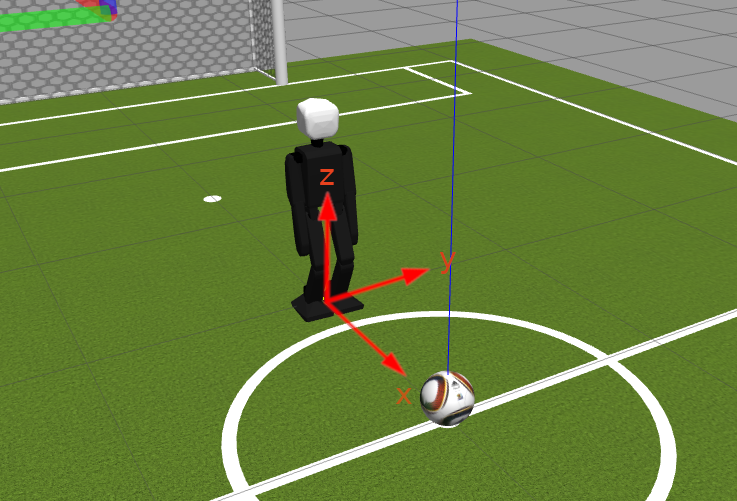
\includegraphics[scale=2]{images/robot_ejes.png}
	\caption{Representación del sistema de referencia usado en el robot.}		
\end{figure}

La cámara está localizada en la cabeza del humanoide, por lo que su centro
de visión se puede representar por un eje que va de la cámara al centroide del 
objeto, en este caso un balón de fútbol.
Para estimar la posición de un objeto que cruce por el centro de visión de la
cámara se necesita establecer un vector unitario:
\[\hat{u} = (u_x, u_y, u_z)\]
conocido en computación gráfica como vector \textit{look at}, (ver figura \ref{fig:LookAt}). Para obtener la ecuación vectorial de la recta paralela al vector \textit{look at} se toma un punto que contenga la recta, en este caso la posición de la cabeza en donde se encuentra la cámara: 

\begin{figure}
	\centering		
	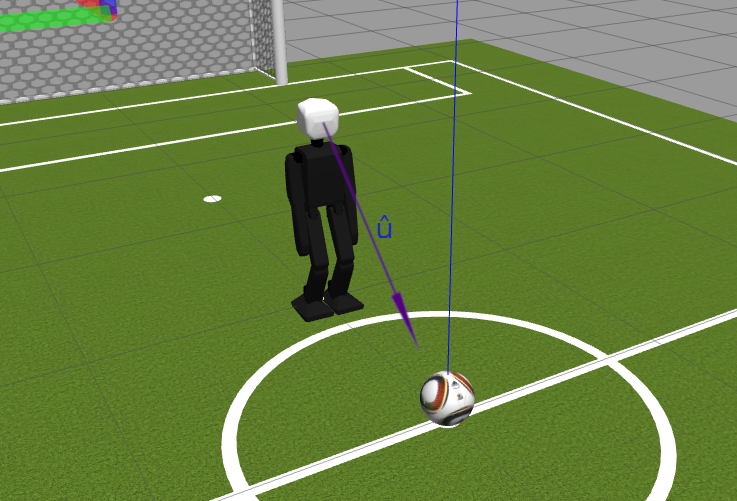
\includegraphics[scale=2]{images/robot_lookat.png}
	\caption{Representación del vector \textit{look at} utilizado en visión computacional.}		
	\label{fig:LookAt}
\end{figure}

\begin{equation}
\label{eq:LookAt}
r(\lambda) = (r_x, r_y, r_z)\quad +\quad \lambda (u_x, u_y, u_z)
\end{equation}


En donde $(r_x, r_y, r_z)$ es la posición en el espacio de la cámara utilizada, referida al sistema de referencia anteriormente mencionado. Se considera que el objetivo siempre estará en el suelo, por lo que el punto de intersección de la ecuación de la recta con el suelo hacen que la variable de altura sea igual a cero, conforme a la siguiente expresión:
\[r = (x, y, 0) = (r_x, r_y, r_z) + \lambda (u_x, u_y, u_z)\]
Despejando $\lambda$ del tercer término de la expresión anterior se obtiene:
\[\lambda = -\frac{r_z}{u_z}\]

De esta manera, substituyendo $\lambda$ en (\ref{eq:LookAt}), se obtiene:
\[x = r_x-\frac{r_z u_x}{u_z}\]
\[y = r_y-\frac{r_z u_y}{u_z}\]

Ya teniendo estas expresiones se procede a sustituir al vector unitario \textit{look at} con coordenadas esféricas, tal y como se observa en la siguiente expresión:
\begin{equation}
\label{eq:LookAtUnitary}
\hat{u}=(u_x, u_y, u_z)=(\sin{ \theta}\cos{\varphi},\sin{\theta}\sin{ \varphi},\cos{\theta})
\end{equation}

Sustituyendo la expresión (\ref{eq:LookAtUnitary}) dentro de los valores $x$ y $y$ quedan como:
\[x=r_x - \frac{r_z \sin{ \theta} \cos{\varphi}}{\cos{\theta}}\]
\[y=r_y - \frac{r_z \sin{\theta} \sin{ \varphi}}{\cos{\theta}}\]

Utilizando la identidad trigonométrica:
\[\tan{\theta} = \frac{\sin{\theta}}{\cos{\theta}}\]

Las ecuaciones para obtener la posición del objetivo siempre y cuando $z=0$ quedan:
\begin{equation}
\label{eq:xBidimentionalPosition}
x=r_x - r_z \tan{\theta}  \cos{\varphi}
\end{equation}

\begin{equation}
\label{eq:yBidimentionalPosition}
y=r_y - r_z \tan{\theta} \sin{\varphi}
\end{equation}

No obstante, el objeto a considerar no es un objeto bidimensional, es un balón con forma esférica que está sobre el plano del suelo, debido a esto se procede a hacer complementar las ecuaciones \ref{eq:xBidimentionalPosition} y \ref{eq:yBidimentionalPosition}, para obtener la posición (x,y,z) del centro del balón.

En la figura \ref{fig:ballProjection}(a) se observa un diagrama del balón en donde el vector \textit{look at} atravieza su centro e intersecta con el suelo en un punto en donde el balón no está. Esto representa un problema, ya que la posición en $x$ sufre una proyección, la cual incrementa mientras el balón tenga mayor radio. A esta proyección se le pondrá la variable $x_c$. Véase la figura \ref{fig:ballProjection}(b)


\begin{figure}
	\centering
	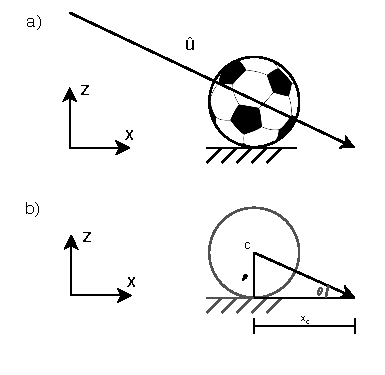
\includegraphics[scale=1.4]{images/ball_projection.pdf}
	\caption{(a) Bosquejo del vector \textit{look at} atravezando el centro del balón esférico; (b) Diagrama de la obtención de la distancia de proyección $x_c$.}
	\label{fig:ballProjection}
\end{figure}

Para obtener la magnitud de $x_c$ es necesario analizar el diagrama de la figura \ref{fig:ballProjection}(b), en donde $\theta$ es el ángulo \textit{pitch} y $\rho$ es el radio del balón. Así se puede obtener la siguiente igualdad:
\[\cot{\theta} = \frac{x_c}{\rho}\]\\

Despejando $x_c$
\[x_c = \rho \cot{\theta}\]

Debido a que $x_c$ se ve afectada también por la posición \textit{yaw} se deducen las siguientes igualdades para corregir el valor de la posición de $x$ y $y$ respectivamente:

\begin{equation}
\label{eq:xcForX}
x_{cx} = \rho \cot{\theta} \cos{\varphi}
\end{equation}

\begin{equation}
\label{eq:xcForY}
x_{cy} = \rho \cot{\theta} \sin{\varphi}
\end{equation}\\

De esta manera, se resta \ref{eq:xcForX}  a \ref{eq:xBidimentionalPosition} y \ref{eq:xcForY} a \ref{eq:yBidimentionalPosition}. Finalmente las ecuaciones resultantes son:

\[x = r_x - r_z \tan{\theta} \cos{\varphi} - \rho \cot{\theta} \cos{\varphi}\]
\[y = r_y - r_z \tan{\theta} \sin{\varphi} - \rho \cot{\theta} \sin{\varphi}\]
\[z = \rho \]


		
	\section{Estimación de estados mediante el Filtro de Kalman}
	Para poder impementar el Filtro de Kalman, se necesita primero tener un modelo matemático del sistema que se pretende tomar mediciones. Analizando el digrama de cuerpo libre de la figura \ref{fig:dynamic_model} se puede hacer un análisis dinámico del balón utilizando la segunda ley de Newton.

\begin{equation}
\sum F = m \ddot{x}
\label{eq:second_law}
\end{equation}

\begin{equation}
F-f_{fricción} = m \ddot{x}
\label{eq:equivalency_1}
\end{equation}

Cambiando el nombre de las variables a corde de nuestro diagrama y tomando en como fuerza de fricción dinámica $f_{fricción} = \mu_d m g $ la igualdad de fuerzas es:
\begin{equation}
F- \mu_d m g = m  \frac{\mathrm{d} \dot{x}}{\mathrm{d} t}
\label{eq:equivalency_2}
\end{equation}
	
Donde $\mu_d$ es el coeficiente de fricción dinámica, $m$ es la masa del balón y $g$ es la aceleración de la gravedad. Dado que ninguna fuerza mas que la de fricción es la que actúa sobre el balón, $F$ se iguala a cero, dejando el modelo el modelo cinemático de la expresión \ref{eq:mathematical_model_1}.

\begin{equation}
\frac{\mathrm{d} \dot{x}}{\mathrm{d} t} = - \mu_d g
\label{eq:mathematical_model_1}
\end{equation}

Despejando la variable $\dot{x}$ para se puede integrar la ecuación para obtener la velocidad en el tiempo $t$ del balón.
\begin{equation}
\int_{\dot{x}_0}^{\dot{x}} \mathrm{d} \dot{x} = -\mu_d g \int_{0}^{t} \mathrm{dt}  
\label{eq:mathematical_model_2}
\end{equation}

Resolviendo la ecuacion \ref{eq:mathematical_model_2} y despejando $\dot{x}$ se puede obtener la siguiente expresión:
\begin{equation}
\dot{x} = \dot{x}_{0} - \mu_d g t 
\label{eq:velocity_prediction}
\end{equation}

Una vez teniendo el modelo para predecir la velocidad del estado siguiente, se procede a integrar nuevamente para obtener su posición:
\begin{equation}
\int_{x_{0}}^{x} \mathrm{dx} = \int_{0}^{t} (\dot{x}_{0} - \mu_d g t) \mathrm{dt}
\label{eq:mathematical_model_4}
\end{equation}

Integrando y despejando $x$ se obtiene:
\begin{equation}
x = x_0 + \dot{x}_0 t - \frac{1}{2} \mu_d g t^2
\label{eq:position_prediction}
\end{equation}

\begin{figure}
\centering
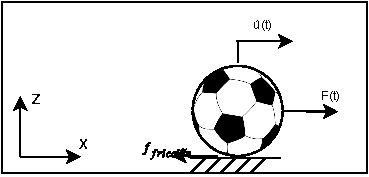
\includegraphics[scale=1.5]{images/dynamic_model.pdf}
\caption{Diagrama de cuerpo libre del objeto de interés}
\label{fig:dynamic_model}
\end{figure}

		\subsubsection*{Descripción del proceso de filtrado en el sistema}
Una vez que se obtuvo el modelo dinámico que describe el movimiento del balón, se procede a escriibir las ecuaciones matriciales que describen al filtro de Kalman (Véase la sección 2.4). De este modo, este filtro es una serie de pasos que iterativamente se deben ir completando de facil cómputo para estimar posiciones y velocidades de un obejeto en movimiento (Figura: \ref{fig:kalman_extended_diagram}).

\begin{figure}
\centering
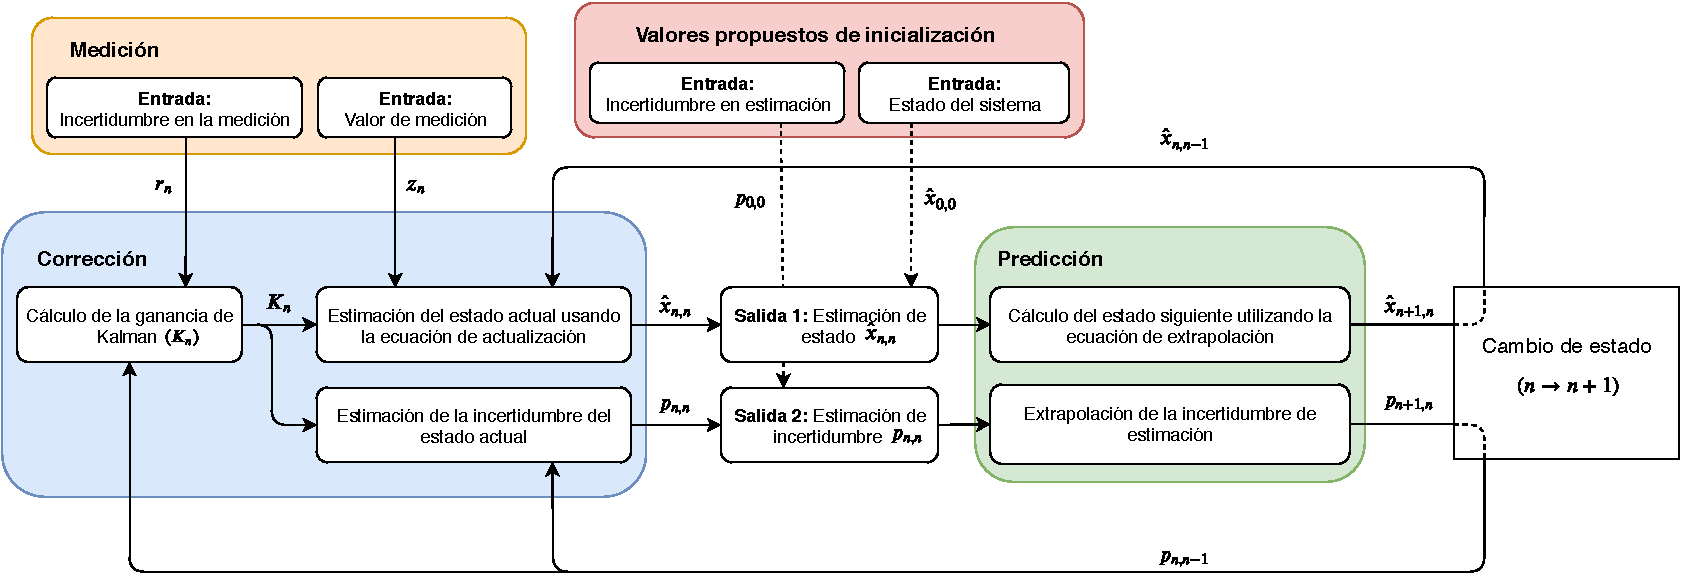
\includegraphics[scale=0.6]{images/kalman_extended_diagram.pdf}
\caption{Diagrama extendidio del funcionamiento paso a paso del Filtro de Kalman}
\label{fig:kalman_extended_diagram}
\end{figure}

		\subsubsection*{Modelado del sistema}
Para desarrollar las ecuaciones de extrapolación de estado se considerará que el balón se desplazará en el suelo sin elevarse o tener rebotes, por lo que el vector de estado $$\hat{x}_n$$ que describe la estimación de posición y velocidad en el plano \textit{(x, y)} es \ref{eq:state_vector}, siguiendo la nomenclatura que se vio en la sección 2.4.

\begin{equation}
\hat{x}_n = \begin{bmatrix}
x_n\\ 
y_n\\ 
\dot{x}_n\\ 
\dot{y}_n
\end{bmatrix}
\label{eq:state_vector}
\end{equation}

Dado que la única fuerza de entrada en el balón es la fricción, la cual depende del coeficiente de fricción dinámica y la gravedad el vector \textit{û} queda representado como:
\begin{equation}
\hat{u}_n = \begin{bmatrix}
-\mu_d g\\
-\mu_d g
\end{bmatrix}
\label{eq:input_signal}
\end{equation}

La matriz de transición \textit{F} es:

\begin{equation}
F = \begin{bmatrix}
1 & 0 & \Delta t & 0\\ 
0 & 1 & 0 & \Delta t\\ 
0 & 0 & 1 & 0\\ 
0 & 0 & 0 & 1
\end{bmatrix}
\label{eq:transition_matrix}
\end{equation}

La matriz de control es:
\begin{equation}
G = \begin{bmatrix}
\frac{1}{2}  \Delta t ^2 & 0 \\ 
0 & \frac{1}{2} \Delta t ^2 \\ 
 \Delta t & 0 \\ 
0 & \Delta t
\end{bmatrix}
\label{eq:control_matrix}
\end{equation}

Por lo tanto, la ecuación de extrapolación de estado es:
\begin{equation}
\hat{x}_{n+1,n} = F \hat{x}_{n,n} + G \hat{u}_{n,n}
\label{eq:extrapolation_equation}
\end{equation}

\begin{equation}
\begin{bmatrix}
x_{n+1,n}\\ 
y_{n+1,n}\\ 
\dot{x}_{n+1,n}\\ 
\dot{y}_{n+1,n}
\end{bmatrix}
=
\begin{bmatrix}
1 & 0 & \Delta t & 0\\ 
0 & 1 & 0 & \Delta t\\ 
0 & 0 & 1 & 0\\ 
0 & 0 & 0 & 1
\end{bmatrix}
\!
\begin{bmatrix}
x_{n,n}\\ 
y_{n,n}\\ 
\dot{x}_{n,n}\\ 
\dot{y}_{n,n}
\end{bmatrix}
+
\begin{bmatrix}
\frac{1}{2}  \Delta t ^2 & 0 \\ 
0 & \frac{1}{2} \Delta t ^2 \\ 
 \Delta t & 0 \\ 
0 & \Delta t
\end{bmatrix}
\!
\begin{bmatrix}
-\mu_d g\\
-\mu_d g
\end{bmatrix}
\end{equation}

El resultado de la multiplicación matricial resulta:
\begin{equation}
\left\{\begin{matrix}
x_{n+1, n} = & x_{n,n} + \dot{x}_{n,n} \Delta t - \frac{1}{2} \mu_d g \Delta t^2\\ 
y_{n+1, n} = & y_{n,n} + \dot{y}_{n,n} \Delta t - \frac{1}{2} \mu_d g \Delta t^2\\ 
\dot{x}_{n+1, n} = & \dot{x}_{n,n} - \mu_d g \Delta t\\ 
\dot{y}_{n+1, n} = &\dot{y}_{n,n} - \mu_d g \Delta t 
\end{matrix}\right.
\end{equation}
	
	\section{Obtencion de los parametros}
		\subsection*{Obtención de la incertidumbre en la estimacion}
	Dado que el proceso de estimación en el Filtro de Kalman es un modelo basdo en la esperanza de una serie de variables aleatorias para obtener el valor "oculto" el cual se considera el real. Este proceso de filtrado considera que todos los errores tanto en medición como en estimación tienen una \textit{distribución normal} por lo que cada incertidumbre tiene que expresarse como la varianza de una recompilación de datos.	
		\subsection*{Obtención de la incertidumbre en la medicion}
		\subsection*{Obtención de la ganancia de Kalman}